\documentclass[a4paper]{article}
\usepackage{pmph_proj}
\usepackage{listings}
\usepackage{appendix}
\usepackage{wrapfig}
\usepackage{graphics}
\usepackage{color}
\definecolor{lightgray}{rgb}{.9,.9,.9}
\newsavebox\lstbox
\newsavebox\lstboxtwo
\newsavebox\lstboxthree
\newsavebox\lstboxfour
\newsavebox\lstboxfive
\header{%
  assignment={Making Woody Parallel},%
  authors={Hugh McGrade <\texttt{wbr412@alumni.ku.dk}>\\
    Mads Obitsø <\texttt{scr411@alumni.ku.dk}>\\
    Titus Robroek <\texttt{robroek@di.ku.dk}>},%
  shortAuthors={\texttt{McGrade, Obitsø, Robroek}},%
  date={\today}
}

\allowdisplaybreaks
\begin{document}
\maketitle

\begin{abstract}
  
\end{abstract}

\section{Introduction}

Random forests have long been a staple of machine learning. They offer a fast, reliable way of tackling classification and regression problems. Their practical ability, however, is not without bounds. Scaling up trees to huge sizes, having massive numbers of trees and processing gigantic numbers of queries all show the limits of current processing technology. This report is about utilising GPU computing to scale up decision tree processing.

In order to utilise GPU computing for decision tree processing we implemented the key part of random forest prediction - the evaluation of a single decision tree with test data - in Woody. This implementation is intended for use as a replacement for the existing decision tree processing in the Woody random forest framework \cite{woody}.

\section{Motivation}

This research aims to investigate ways to scale decision trees up. Larger decision trees may be very useful for some areas of research. The field of Remote Sensing, for example, has vast amounts of data to be --------ADD MORE---------------

\section{Woody Random Forest Prediction in Futhark}

\subsection{Decision tree evaluation}

The evaluation of a single decision tree in a random forest prediction takes a single decision tree from the forest and a matrix of test data. From this a vector of predictions is produced, each of which corresponds to the decision made from evaluating the decision tree for a given row of the test data. These rows can either be specified by an indices array mapping decision indices to row indices, or simply by taking each row in order.

\begin{wrapfigure}{R}{0.3\textwidth}
\centering
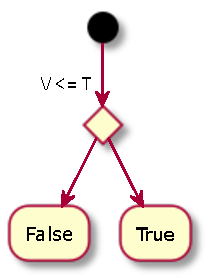
\includegraphics[width=0.25\textwidth]{decision_node.pdf}
\caption{\label{fig:frog1}This is a figure caption.}
\end{wrapfigure}

Each node of the decision tree specifies a threshold for proceeding on its left or right branch and the feature (column of the test data) which should be used to evaluate this threshold. In evaluation this continues until a leaf node is reached which is then the result. 

\subsection{Interoperation of Woody and Futhark}

The Futhark compiler features code generation for the PyOpenCL library, allowing Futhark code compiled for OpenCL to be called from Python. This generated code accepts NumPy arrays as Futhark arrays. As Woody is written in Python, we are able to compile our Futhark library for PyOpenCL and use it as a library in Woody's Python code.

\subsection{Tree and test data encoding for Futhark}

In order to pass the tree and test data from Woody to Futhark, we encoded each as a series of flat arrays.

In the case of the tree, this took the form of four arrays giving the properties of each node by index: \texttt{treeLeftid}, \texttt{treeRightid}, \texttt{treeFeature} and \texttt{treeThres\_or\_leaf}. These give the left child ID, right child ID, feature index and threshold respectively.

The test data matrix is described by a single array containing each of the test values (\texttt{Xtest}) and values \texttt{nXtest} and \texttt{dXtest} which give the shape of the matrix.

\subsection{Basic Futhark implementation}


\begin{figure}
\centering
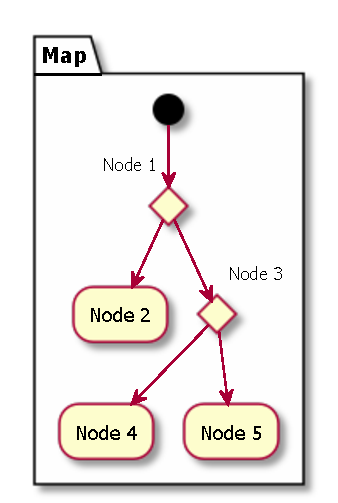
\includegraphics[width=0.4\textwidth]{tree_basic.pdf}
\caption{\label{fig:frog1}This is a figure caption.}
\end{figure}
    
We started by producing a translation of Woody's single tree query into Futhark. Woody's version is parallelised using OpenMP over the trees in the forest. The Futhark for this is as follows:

\vspace{1ex}
\begin{lrbox}{\lstbox}
\begin{minipage}{\textwidth}
\begin{lstlisting}[language=Haskell, breaklines]
  unsafe map (\ i ->
  let idx = if dindices > 0 then indices[i] else i
  let row_start = idx * dXtest
  in loop node_id = TREE_ROOT_ID
        while treeLeftid[node_id] != TREE_CHILD_ID_NOT_SET do
              if Xtest[row_start + treeFeature[node_id]] <= treeThres_or_leaf[node_id]
                then treeLeftid[node_id]
                else treeRightid[node_id]
             ) (iota n_preds)
\end{lstlisting}
\end{minipage}
\end{lrbox}  
\vspace{1ex}

\colorbox{lightgray}{\usebox\lstbox}

This implementation parallelises the evaluation over the rows of the test data using a map over each prediction. The function to be mapped uses a Futhark while loop which assigns the root of the tree to \texttt{node\_id} and subsequently the result of the loop body which gives the next node. The loop terminates when a leaf node is reached and thus the function returns the ID of the leaf node.

TODO: discussion of this algorithm in Futhark

Woody's original C implementation of this algorithm, with comments added, can be found in appendix A.

\subsection{Flat Futhark implementation}

\begin{figure}
\centering
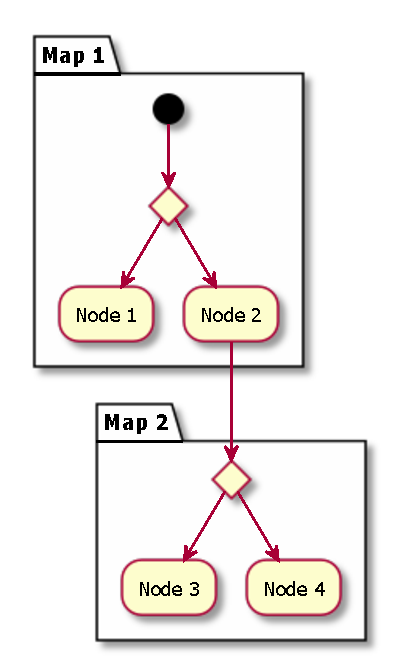
\includegraphics[width=0.4\textwidth]{tree_flat.pdf}
\caption{\label{fig:frog1}This is a figure caption.}
\end{figure}

A different approach to parallelising tree querying in Futhark is to flatten the basic implementation's \texttt{map} and \texttt{while} loop into a single \texttt{map} and repeating this sequentially for each layer of the tree. This is achieved by joining the nodes array and data array

\vspace{1ex}
\begin{lrbox}{\lstboxtwo}
\begin{minipage}{\textwidth}
\begin{lstlisting}[language=Haskell, breaklines]
loop node_array for row in iota(depth) do
    unsafe map (\ (node_id, data_row_start) ->
                 if (treeLeftid[node_id] != 0)
                    then (if Xtest[data_row_start + treeFeature[node_id]] <= treeThres_or_leaf[node_id]
                        then treeLeftid[node_id]
                        else treeRightid[node_id])
                    else node_id)
                    (zip node_array data_row_starts)
\end{lstlisting}
\end{minipage}
\end{lrbox}
\vspace{1ex}

\colorbox{lightgray}{\usebox\lstboxtwo}

\subsection{Pruning Futhark implementation}

Our semi-flat futhark implementation applies a map for every layer of the tree. Some queries, however, will have hit a leaf at some point. The current implementation, however, still attempts to apply a map for every query, even if it has stopped at a leaf. Our next implementation attempts to solve this issue.
We want to avoid processing paths that are stuck on a leaf node over and over again. We do this by applying a filter operation on our iterations. We filter the queries based on them being on a leaf node or not. This causes the map to only be applied of "live" paths.
We use a transposition array in order to track the shape of our current data. After the loop over the rows, this array is used to revert the data into it's original shape. This allows us to retrieve the correct data objects.

\vspace{1ex}
\begin{lrbox}{\lstboxthree}
\begin{minipage}{\textwidth}
\begin{lstlisting}[language=Haskell, breaklines]
  let nodes = zip node_array data_row_starts
  let leaves = []
  let (_, leaves) = loop (nodes, leaves) for row in iota(depth) do
                    let new_nodes = (unsafe map next_node nodes)
                    in (unsafe filter is_not_leaf new_nodes,
                        leaves ++ (unsafe filter is_leaf new_nodes))
  let result = map (\ (a, _) -> a)
                    (radix_sort_by_key (\ (_, a) -> a) 
                                        i32.num_bits
                                        i32.get_bit
                                        leaves)
  in result
\end{lstlisting}
\end{minipage}
\end{lrbox}
\vspace{1ex}

\colorbox{lightgray}{\usebox\lstboxthree}

This implementation again parallelises the queries by applying a map to each row. As it prunes the tree we can expect it to perform better on larger, deeper and less balanced trees. 

\subsection{Treesolver Precompute}

A further approach we took to implement decision tree querying in Futhark was to compute the outcome of each tree node prior to traversing the tree. This greatly increases the scope for parallelism in the evaluation of tree thresholds as every node can now be computed independently. To do this we map the function \texttt{make\_next\_tree} (with the tree) to every row of the data. This further maps the function \texttt{next\_node} (with the row of the data) to every node of the tree, creating an array which for each node (by index) gives the following node's index. The tree is then trivially traversed by following these pointers from the root node.

\vspace{1ex}
\begin{lrbox}{\lstboxfour}
\begin{minipage}{\textwidth}
\begin{lstlisting}[language=Haskell, breaklines]
let next_node
  (row: []f64)
  ((left, right, feature, thres) : (i32, i32, i32, f64)) : i32 =
  if row[feature] <= thres then left else right

let make_next_tree
   (tree: [](i32, i32, i32, f64))
   (row : []f64) : []i32 =
   map (next_node row) tree

let traverse
   (next_nodes: []i32): i32 =
   let (last, current) = (0, next_nodes[0])
   let (result, _) = loop (last, current) while current != 0 do (current, next_nodes[current])
   in result
   
let nodes = zip4 treeLeftid treeRightid treeFeature treeThres_or_leaf
let rows = unflatten nXtest dXtest Xtest

let next_nodes = unsafe map (make_next_tree nodes) rows

in unsafe map traverse next_nodes
   
\end{lstlisting}
\end{minipage}
\end{lrbox}
\vspace{1ex}

\colorbox{lightgray}{\usebox\lstboxfour}

We found this approach was far better suited to using an idiomatic Futhark style and made the potential for parallelisation clearer by separating tree travsersal. Future work could consider better flattening this approach.

\subsection{Super flat}

\vspace{1ex}
\begin{lrbox}{\lstboxfive}
\begin{minipage}{\textwidth}
\begin{lstlisting}[language=Haskell, breaklines]
let repeated_criteria = flatten (replicate nXtest treeFeature)
  let repeated_offsets = flatten (map (\ i -> replicate treelength i) (steps 0 nXtest dXtest))
  let flcr = map2 (+) repeated_offsets repeated_criteria
  let scattered_features = unsafe map (\ i -> Xtest[i]) flcr
  let threshold_result = map2 (<=) scattered_features (flatten (replicate nXtest treeThres_or_leaf))
  let left_or_right = (\ b l r -> if b then l else r)
  let repeatedLeft = flatten (replicate nXtest treeLeftid)
  let repeatedRight = flatten (replicate nXtest treeRightid)
  let directions = map3 left_or_right threshold_result repeatedLeft repeatedRight

  in unsafe map traverse (unflatten nXtest treelength directions)
\end{lstlisting}
\end{minipage}
\end{lrbox}
\vspace{1ex}

\colorbox{lightgray}{\usebox\lstboxfive}


\section{Experimental Setup}

To evaluate our Futhark implementation, we performed various comparisons with the 

All experiments were performed on a GPU node with two Intel(R) Xeon(R) CPU E5-2650 v2 processors at 2.60GHz (32 cores, 2 threads per core) and two GeForce GTX 780 Ti graphics cards.

TODO: Describe the data

\section{Evaluation}

\section{Conclusion}

\begin{thebibliography}{}

\bibitem{woody}
Gieseke, Fabian, and Christian Igel. "Training Big Random Forests with Little Resources." arXiv preprint arXiv:1802.06394 (2018).

\end{thebibliography}

\appendix
\section{Woody single tree query in C}
\begin{lstlisting}[language=C,breaklines]
void cpu_query_tree(TREE tree, FLOAT_TYPE *Xtest, int nXtest, int dXtest,
FLOAT_TYPE *predictions, int *indices, int dindices, int prediction_type) {

  // start from root
	register TREE_NODE *node = tree.root;

  // tpatt = pointer to the start of the current row of the test data
	register FLOAT_TYPE *tpatt;

  // i = prediction index
  // node_id = id of the current node
  // idx = row of the test data to be used for the current prediction
	register unsigned int i, node_id, idx;

  // if no indices are given, make as many predictions as there are rows in the test data
	int n_preds = nXtest;
	if (dindices > 0) {
    // If indices are given, make as many predictions as there are indices
		n_preds = dindices;
	}
	for (i = 0; i < n_preds; i++) {
		if (dindices > 0) {
      // If there are indices, use their index for row of the current prediction
			idx = indices[i];
		} else {
      // Otherwise use the index of the current prediction
			idx = i;
		}

		tpatt = Xtest + idx * dXtest;
    // node_id = ID of the root node
		node_id = TREE_ROOT_ID;

    // Loop until a leaf node is reached
		while (node[node_id].left_id != TREE_CHILD_ID_NOT_SET) {
      // If test value taken from (idx, node.feature) where node is the current node
      // is less than or equal to the node.thres_or_leaf
			if (tpatt[node[node_id].feature] <= node[node_id].thres_or_leaf) {
        // Take the left child
				node_id = node[node_id].left_id;
			} else {
        // Take the right child
				node_id = node[node_id].right_id;
			}
		}

		if (prediction_type == PREDICTION_TYPE_NORMAL) {
			predictions[i] = node[node_id].thres_or_leaf;
		} else if (prediction_type == PREDICTION_TYPE_LEAVES_IDS) {
			predictions[i] = (FLOAT_TYPE) node_id;
		} else {
			printf("Error: Unknown prediction type: %i ", prediction_type);
			exit(EXIT_FAILURE);
		}

	}

}
\end{lstlisting}

\end{document}
